%%%%%%%%%%%%%%%%%%%%%%% file template.tex %%%%%%%%%%%%%%%%%%%%%%%%%
%
% This is a template file for Web of Conferences Journal
%
% Copy it to a new file with a new name and use it as the basis
% for your article
%
%%%%%%%%%%%%%%%%%%%%%%%%%% EDP Science %%%%%%%%%%%%%%%%%%%%%%%%%%%%
%
%%%\documentclass[option]{webofc}
%%% "twocolumn" for typesetting an article in two columns format (default one column)
%
\documentclass{webofc}
\usepackage[varg]{txfonts}   % Web of Conferences font

\usepackage[sorting=none]{biblatex}
\usepackage{hyperref}
\addbibresource{bibliography.bib}
%
% Put here some packages required or/and some personnal commands
%
%
\begin{document}

%
\title{dCache integration with CERN Tape Archive}
%
% subtitle is optionnal
%
%%%\subtitle{Do you have a subtitle?\\ If so, write it here}

\author{
         \firstname{Tigran} \lastname{Mkrtchyan}\inst{1}\fnsep\thanks{\email{tigran.mkrtchyan@desy.de}} \and
        \firstname{Jacek} \lastname{Chodak}\inst{1}\fnsep \and
        \firstname{Mwai} \lastname{Karimi}\inst{1}\fnsep \and
        \firstname{Ralf} \lastname{Lueken}\inst{1}\fnsep \and
        \firstname{Svenja} \lastname{Meyer}\inst{1}\fnsep \and
        \firstname{Peter} \lastname{Suchowski}\inst{1}\fnsep \and
        \firstname{Christian} \lastname{Voss}\inst{1}\fnsep
}

\institute{
   \affil{
       \orgname{Deutsches Elektronen-Synchrotron DESY}, \orgaddress{\street{Notkestrasse 85}, \postcode{22607} \city{Hamburg}, \country{Germany}}
       }
}

\abstract{%
  The ever-increasing amount of data that is produced by modern scientific facilities like EuXFEL or LHC puts
  high pressure on the data management infrastructure at the laboratories. This includes poorly shareable resources
  of archival storage, typically, tape libraries. To achieve maximal efficiency of the available tape resources a
  deep integration between hardware and software components is required.

  The CERN Tape Archive (CTA) is an open-source storage management system developed by CERN to manage LHC experiment
  data on tape. Although today CTA's primary target is CERN Tier-0, the data management group at DESY considers the
  CTA is a main alternative to commercial HSM systems.

  dCache has an extensible tape interface that allows connectivity almost to any tape system. Together with the CERN
  Tape Archive team we are working on seamless integration of CTA into dCache.

  This work shows the design of dCache-CTA integration, its current status and its first deployment experience at DESY.
}
%
\maketitle
%
\section{Introduction}
\label{intro}

The ever-increasing amount of data that is produced by modern scientific facilities like EuXFEL or LHC puts high pressure
on the data management infrastructure at the laboratories. The challenges that have to be addressed span over the full data 
life-cycle: from ingest, efficient data analysis, up to long-term preservation. The latter typically utilizes magnetic
tape media, which in combination with disk storage covers the data management requirements. DESY-IT groups use dCache\cite{dcache}, a
storage system developed at DESY in collaboration with Fermilab and Nordic eInfrastructure Collaboration (NeIC), to manage
large numbers of disk servers and transparent data migration to and from archival storage.

Even though today large hard disk-based storage systems are cost, space and volume-effective (1 PB disk storage requires less than a ${1m^{3}}$ of space),
magnetic tapes are still the best option for long-term data archival, especially for so-called cold data, data that is rarely accessed.
Indeed, tape cartridges don't require electric power when not used, can store up to 20TB of uncompressed data and are designed for
15 - 30 years of archival storage. To organize a large number of tape cartridges, tape libraries with robotic arms are used.

There are, of course, some downsides of tape-based technologies. Though, when streaming a modern tape drive provides up to 400 MB/s,
the so-called positioning time on average is about 50 seconds. This doesn't include the mount time, the time which is needed by the
robotic arm to put the tape into an appropriate tape drive. Moreover, magnetic tapes don't support concurrency, which means that only
one stream, e.g. only one file, can be read or written at any point in time.

Thus, to achieve maximal efficiency of the available tape resources, e.g. maximize the time during which tape is read or written and
maximal speed, a deep integration between hardware and software components is required.

Since the early 90's DESY-IT has been relying on Open Storage Manager (OSM) software to operate tape libraries and access data on tapes.
During these three decades, the OSM underwent many changes. Over 80\% of the original code base has been updated to address computer, network,
operating system and software paradigms that have changed over decades. Nevertheless, the scaling capabilities put into the original design
don't apply today. Moreover, the commercial software license of OSM doesn't allow us to share our changes with the broader scientific community.
Thus, a new scalable and preferably open-source success is required.

With dCache as the primary disk layer in front of an HSM, the tape system should fulfill the following requirements:

\begin{itemize}
    \item Maximize tape HW efficiency
    \item Integration into DESY ecosystem
    \item Integration with dCache tape interface
    \item Support Enterprise \& LTO
    \item Daily turnover about 1PB
    \item Stable operation for the next decade
    \item Should be Open-source, adopting open standards
    \item Wide user and technology community
    \item State-of-the-art integration/use development tools (CI/CD)
\end{itemize}

\section{Cern Tape Arcive}
\label{sec:cta}

The CERN Tape Archive (CTA)\cite{cta} is an open-source storage system developed by the CERN IT storage group to
replace the legacy CASTOR system that is used to manage experiments data on tape. Its architecture is designed
to meet the requirements of LHC Run 3 as well as HL-LHC, thus needing the most data-intensive scientific workloads.

The CTA has two key components: frontend and tape daemon\ref{fig:cta_overview}. The frontend accepts the requests, like archive, retrieve, delete or cancel, from the attached disk storage and puts them into the request queue. If needed, the file catalog is updated. The scheduling logic is embedded into the tape daemons, which are per-tape drive processes and seek matching tasks in the request queue. Once the desired number of requests is collected, the data is moved  between disk and tape media.

\begin{figure}
    \centering
    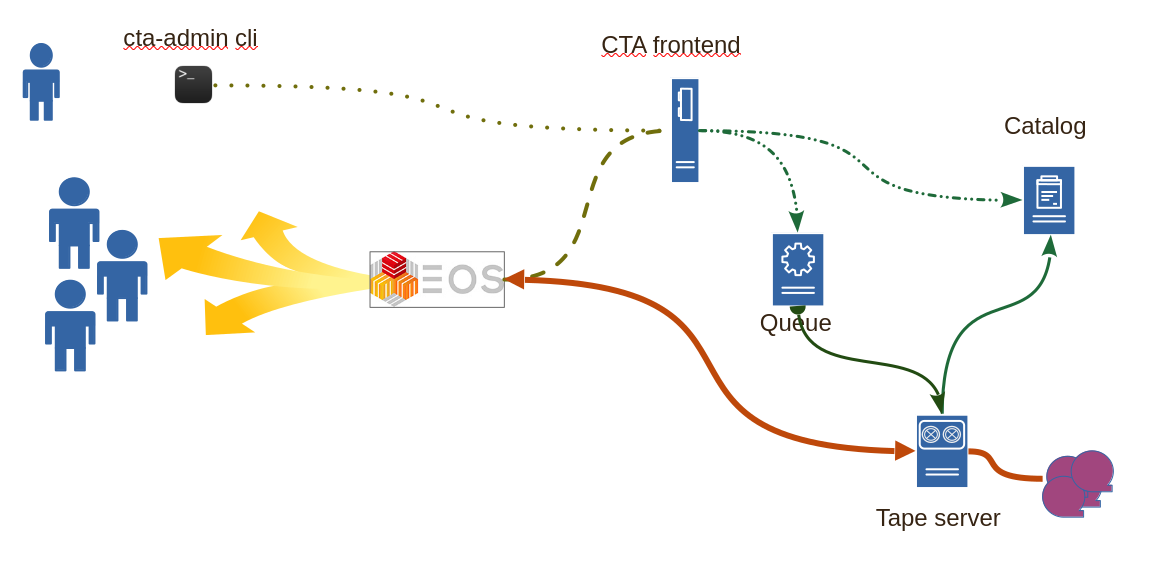
\includegraphics[scale=0.25]{cta-design.png}
    \caption{CTA design overview}
    \label{fig:cta_overview}
\end{figure}

Out of the box, CTA comes with a frontend that communicates with EOS, the disk system deployed at CERN. However, as CTA's queuing system is not EOS aware, other frontend implementations are possible.

\section{dCache Integration with CTA}
\label{sec:integration}

dCache has a flexible tape interface which allows connectivity to any tape system. There are two ways that a file can be migrated to tape. Ether dCache calls a tape system specific copy command or through interaction via an in-dCache tape system specific driver, called a nearline storage provider. The latter has been shown (by NDGF, TRIUMF and KIT Tier-1s), to provide better resource utilization and efficiency\cite{endit_kit}. Thus, for seamless integration of CTA the dCache developers at DESY have implemented CTA specific nearline storage provider, called dcache-cta, and a corresponding frontend component for CTA. The communication between dCache and the new forntend is based on Google’s gRPC library.

\begin{figure}
    \centering
    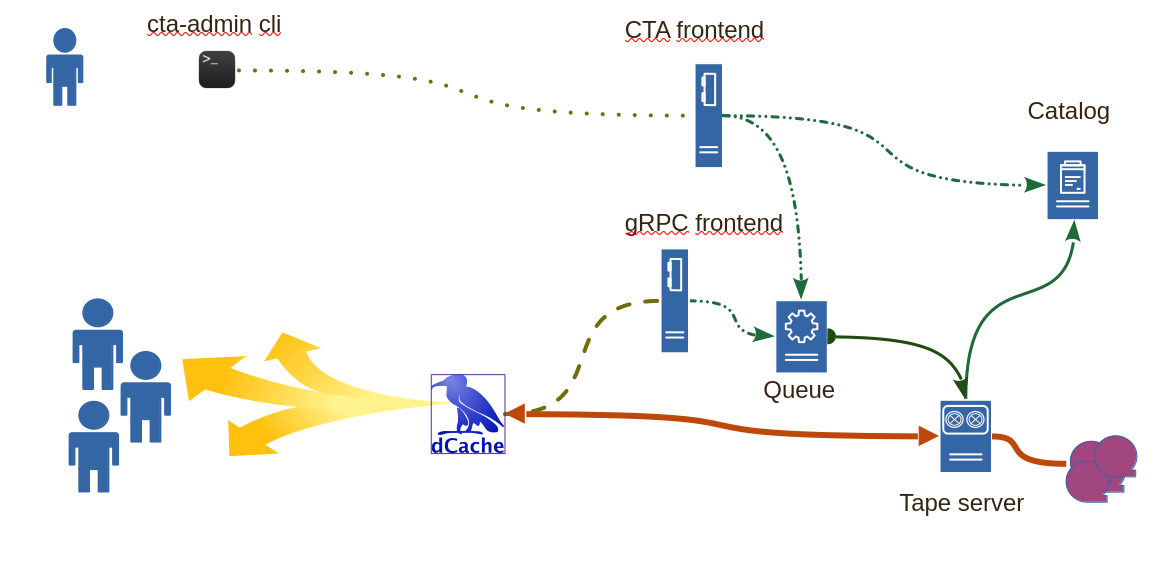
\includegraphics[scale=0.25]{dcache-cta-integration.png}
    \caption{dCache integration with CTA}
    \label{fig:dcache_integration}
\end{figure}

\newpage
\section{Bibliography}
\label{refs}
\printbibliography

\end{document}
